\subsubsection{Descripción y topología de los paquetes}

lugar, dia de la semana, hora aproximada, fecha, wifi o ethernet
cantidad de paquetes tomados, tiempo de muestreo

Nuestro segundo experimento consistió en capturar los paquetes de la LAN Wi-Fi de la empresa Honeywell. En esta red no hay mucho tráfico, ya que la mayoría de las computadores se conectan via Ethernet a una VPN. Esta red es dedicada a transacciones que no necesiten un nivel de seguridad. La captura se realizo un día lunes a las 11 am. durante media hora, lográndose capturar 253 paquetes.  

grafico del grafo de la red

\begin{figure}[H]
 \begin{center}
  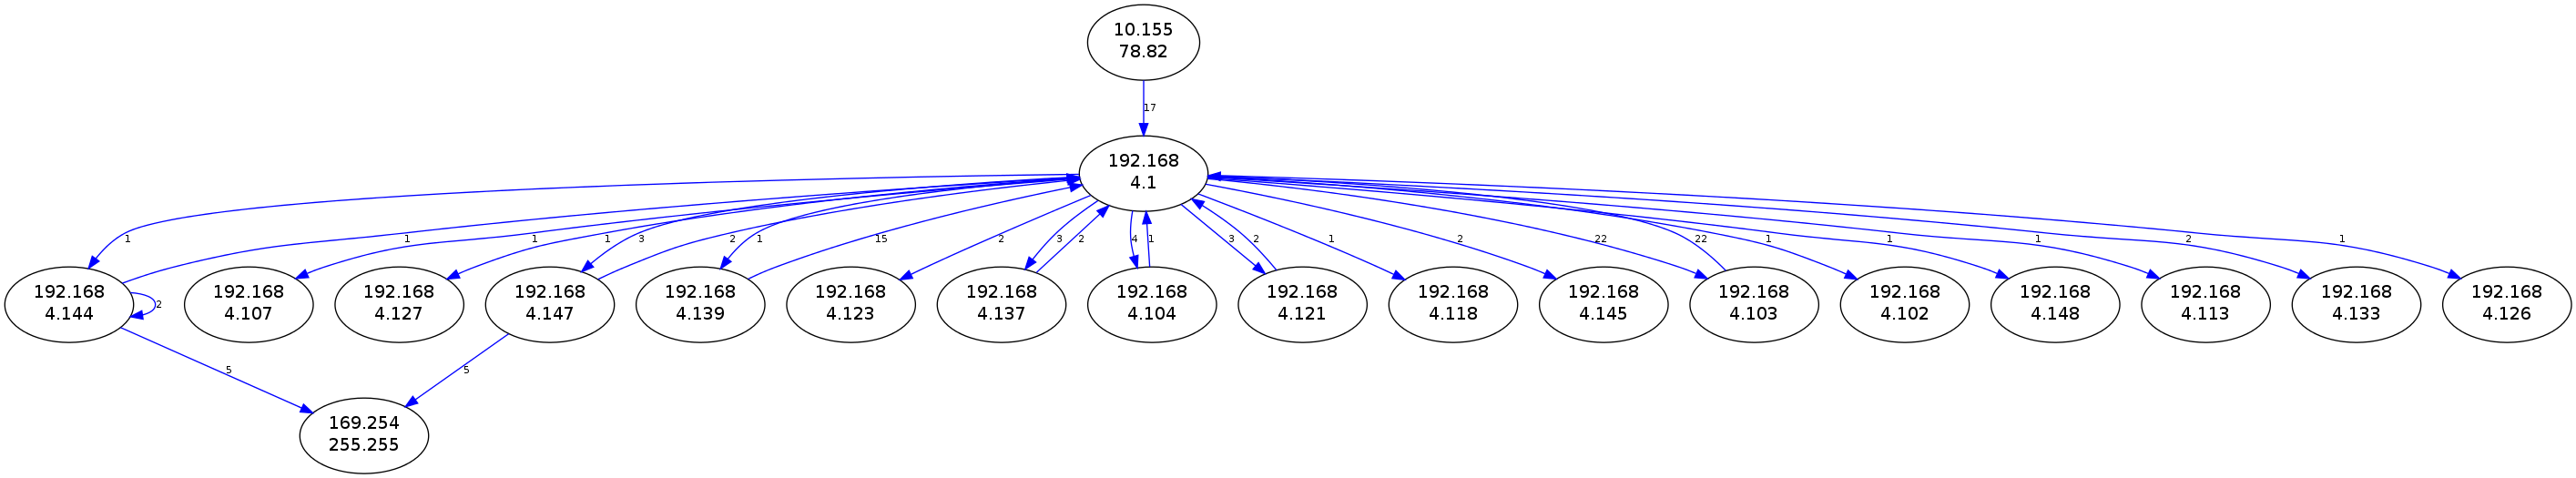
\includegraphics[width=\linewidth]{../imgs/prueba_laburo-ips_red.png}
  \caption{Medición Honeywell}
 \end{center}
\end{figure}


\subsubsection{Fuente: $S_{dst}$}

\begin{figure}[H]
   \begin{minipage}{0.5\linewidth}
     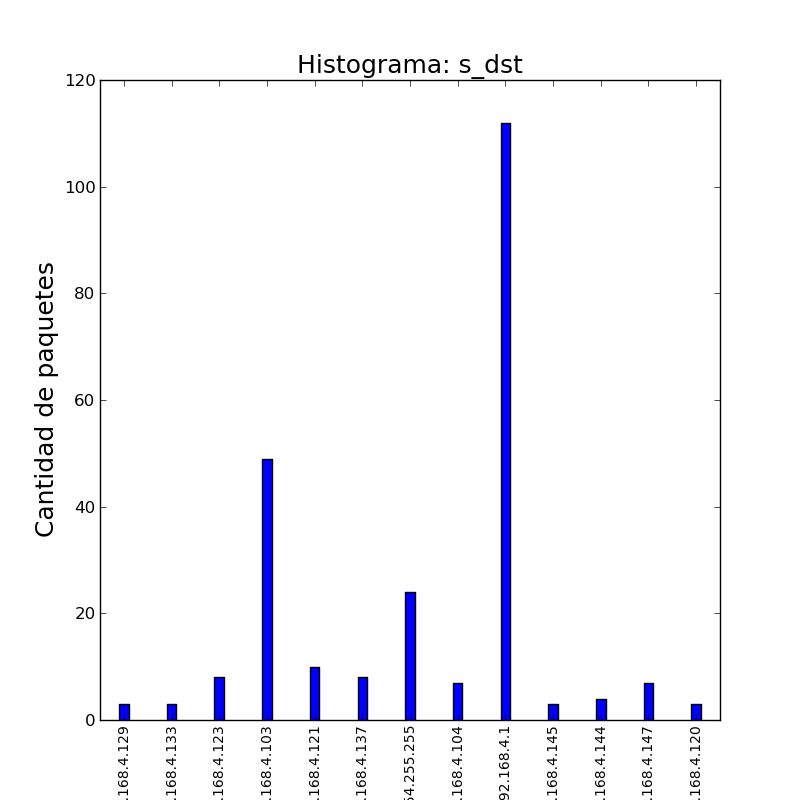
\includegraphics[width=\linewidth]{../imgs/prueba_laburo-ips_s_dst_hist.png}
     \caption{Medición Honeywell}\label{fig:Honeywell-dst-hist}
   \end{minipage}
  \hfill
   \begin{minipage}{0.5\linewidth}
     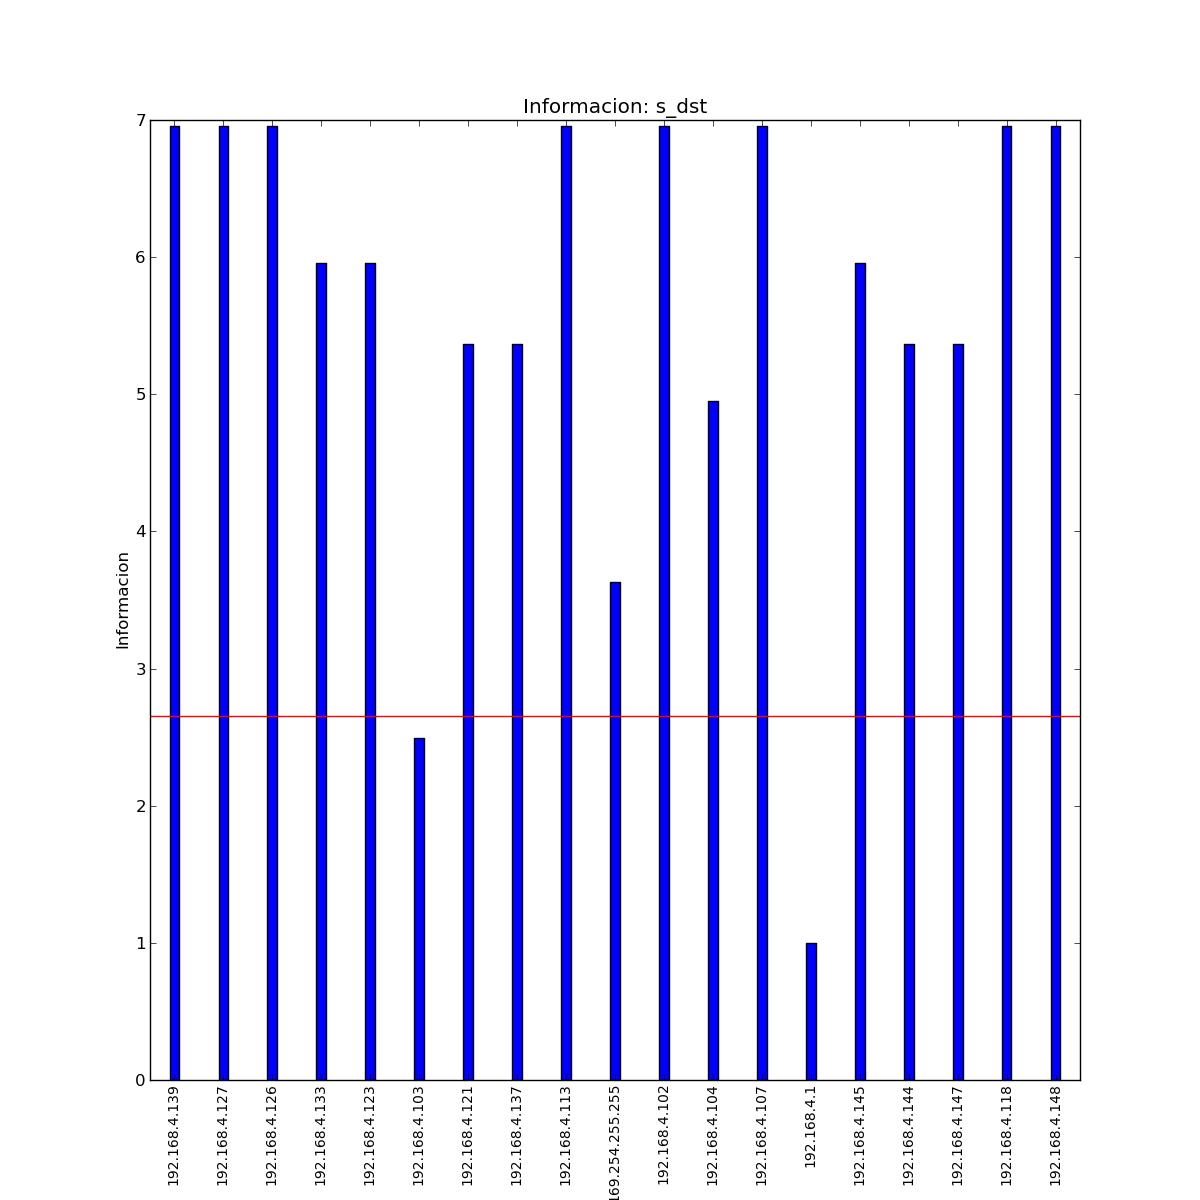
\includegraphics[width=\linewidth]{../imgs/prueba_laburo-ips_s_dst_info.png}
     \caption{Medición Honeywell}\label{fig:Honeywell-dst-info}
   \end{minipage}
 \end{figure}

histograma
grafico de informacion
entropía total

\subsubsection{Fuente: $S_{src}$}

histograma
grafico de informacion
entropía total

\begin{figure}[H]
   \begin{minipage}{0.5\linewidth}
     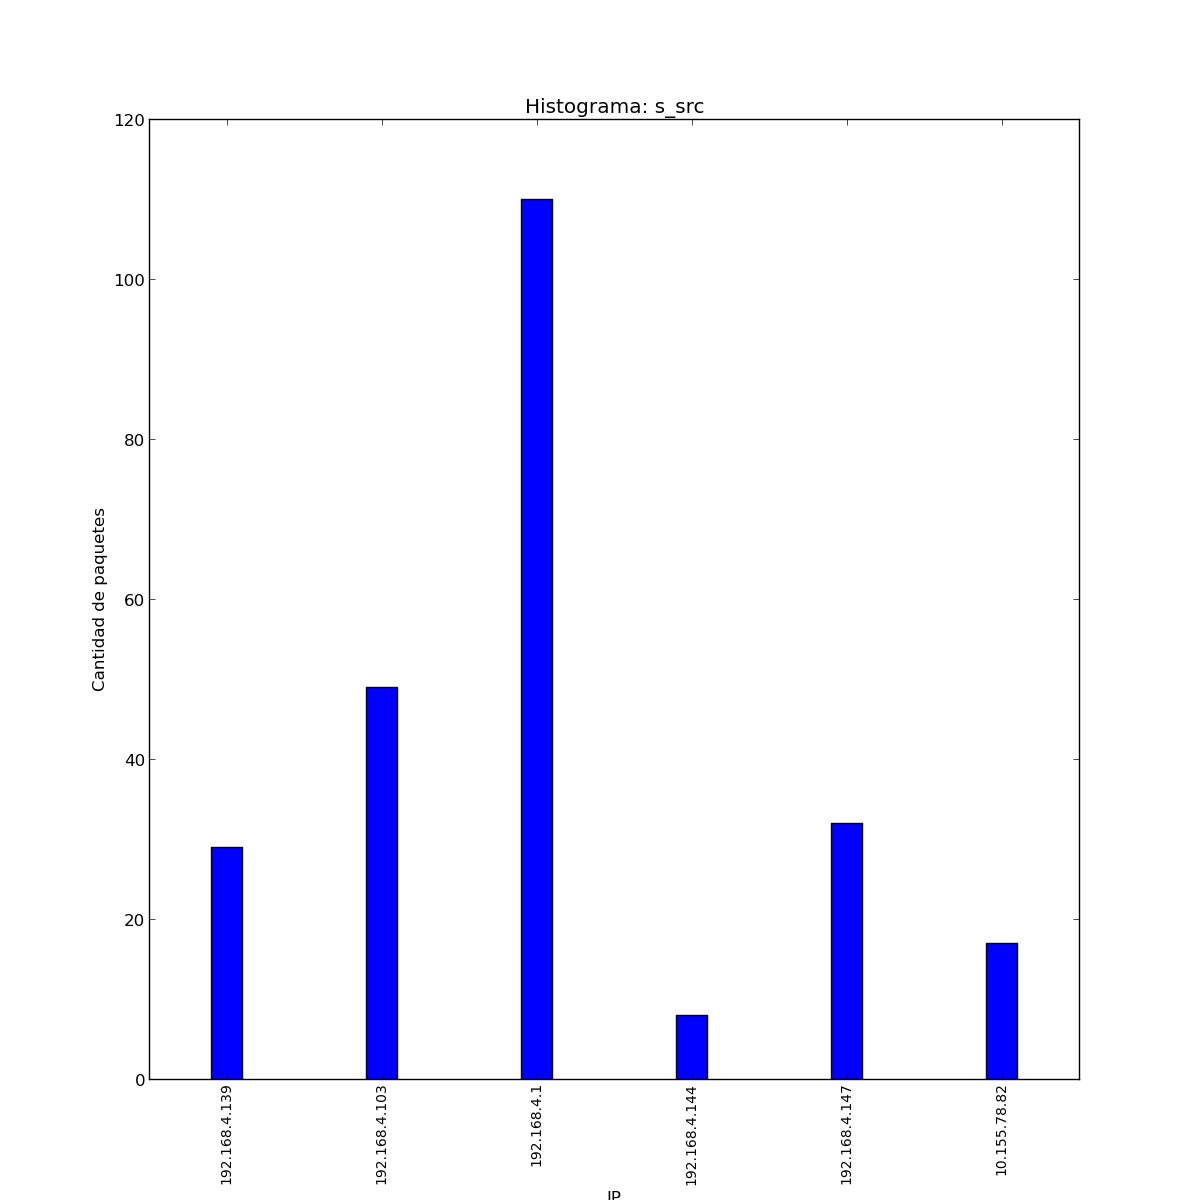
\includegraphics[width=\linewidth]{../imgs/prueba_laburo-ips_s_src_hist.png}
     \caption{Medición Honeywell}\label{fig:Honeywell-src-hist}
   \end{minipage}
  \hfill
   \begin{minipage}{0.5\linewidth}
     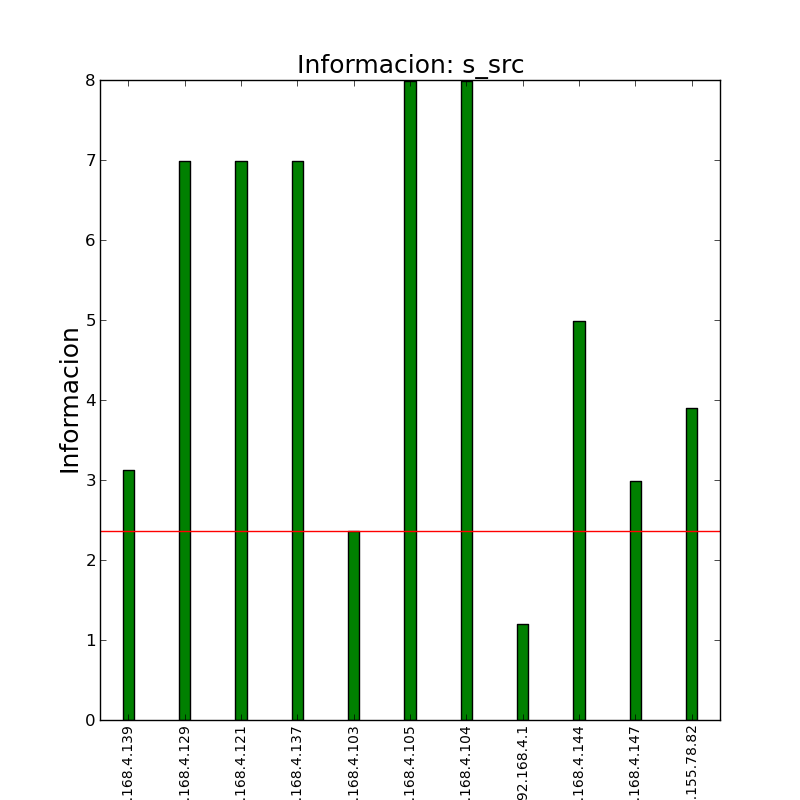
\includegraphics[width=\linewidth]{../imgs/prueba_laburo-ips_s_src_info.png}
     \caption{Medición Honeywell}\label{fig:Honeywell-src-  info}
   \end{minipage}
 \end{figure}

\subsubsection{Discusión}

cualquier cosa interesante sobre este caso en particular